\documentclass[12pt]{article}
 
\newenvironment{sol}[1][Solution]{\begin{trivlist}\item[\hskip\labelsep {\bfseries #1:}]}{\end{trivlist}}
\usepackage{minted}
%\usemintedstyle{perldoc}
\usemintedstyle{vs}
\usepackage{graphicx}
\graphicspath{./}

\usepackage[margin=1in]{geometry} 
\usepackage{amsmath,amsthm,amssymb}
\usepackage{times,url}
\usepackage{tikz}
\usepackage{color}
\usepackage{enumerate}
\begin{document}
\renewcommand{\qedsymbol}{\filledbox}
\begin{center}
    \textbf{CS 5/7350 - Test\#1} \\
    \textbf{October 5, 2022}
%replace X with the appropriate number
\end{center}
\begin{flushright}
Name: \underline{Bingying Liang }\\
ID:  \underline{\ \ \ \ \ 48999397 \ \ \ \ \ }
\end{flushright}

\begin{enumerate}
    \item \ [6 pts] Argue that the problem, S, of sorting an unsorted array of integers of length greater than $100$ elements is at least as hard- and maybe even harder - within a constant factor of $O(1)$ than the problem, L, of finding the three largest elements of the same unsorted array of integers.
    \begin{sol}
        Since a solver for S can be used to solve L by sorting the array and then printing the last 3 elements, problem S must be just as hard or possible harder than Problem L.
    \end{sol}
    \item \ [6 pts] What is an algorithm?
    \begin{sol}
    Informally, an algorithm is any well-defined computational procedure that takes some value, or set of values, as input and produces some value, or set of values, as output in a finite amount of time. An algorithm is thus a sequence of computational steps that transform the input into the output. An algorithm can be viewed as a tool for solving a well-specified computational problem. The statement of the problem specifies in general terms the desired input/output relationship for problem instances, typically of arbitrarily large size. The algorithm describes a specific computational procedure for achieving that input/output relationship for all problem instances.\\
    \textcolor{red}{A step-by-step procedure for solving a problem in a finite amount of time.}
    \end{sol}

    % 3
    \item \ [5 pts] Draw two different trees where both trees have a pre order traversal of ABC and a post order traversal of CBA.
    \begin{sol}
    \hspace*{\fill}\\
    \begin{enumerate}
        \item 
        \begin{align*}
        \begin{tikzpicture}
        \node{A}
        child{node{B}
              child {node{C}
              }
              child[missing]
            }
        child[missing];
        \end{tikzpicture}
        \end{align*}

        \item
        \begin{align*}
        \begin{tikzpicture}
            \node{A}
            child[missing]
            child{
                node{B}
                    child{
                        node{C}
                    }
                    child[missing]
            };
        \end{tikzpicture}
        \end{align*}
        \end{enumerate}

        \textcolor{red}{---------------------------------------------------------------------------------------------------------------}
        \begin{align*}
            \begin{tikzpicture}
                \node{A}
            child[missing]
            child{
                node{B}
                    child[missing]
                    child{
                        node{C}
                    }
            };
            \end{tikzpicture}
        \end{align*}
        \textcolor{red}{---------------------------------------------------------------------------------------------------------------}
    \end{sol}

    % 4
    \item \ [5 pts] Using $n_0$ equal to 10, show that $f(n) = 8n^2+5n+1$ is $\Omega(n)$
    \begin{sol}
    \begin{align*}
        & 0 \leq c_1n \leq 8n^2 + 5n +1, \forall v \geq 10 \\
        & 0 \leq c_1 \leq 8n + 5 + \frac{1}{n}, \forall v \geq 10 \\
        & c_1 \text{ can be } 80. \\
        &\text{Note } 80 \text{ is not the tightest value, but is always less than } 8n + 5 + \frac{1}{n}
    \end{align*}
    \end{sol}

    % 5 
    \item \ [8 pts] You run different programs for various values of "n" and create 4 tables of runtimes. Give the Asymptotic bounds that each of the tables support?
    \begin{center}
        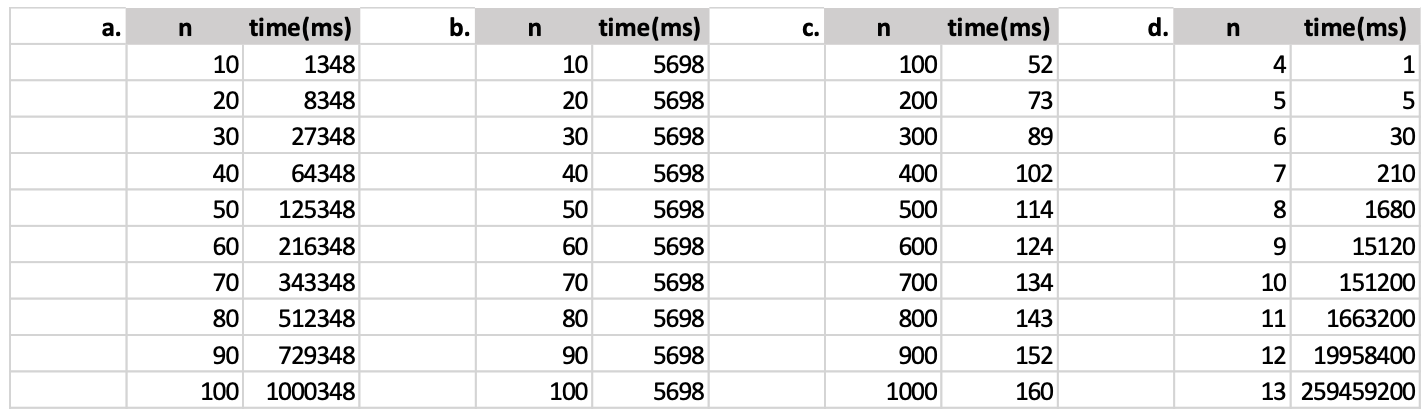
\includegraphics[width=0.9\textwidth]{p1.png}.
    \end{center}
    \begin{sol}
    \begin{enumerate}
        \item $\Theta(n^3)$
        \begin{align*}
            \frac{n_2}{n_1}=\frac{80}{40} = 2, \frac{f(n_2)}{f(n_1)}=\frac{512346}{64348} \approx 7.96 \approx 8 = 2^3
        \end{align*}

        \item $\Theta(1)$
        \begin{align*}
            \frac{n_2}{n_1} = \frac{80}{40} = 2, \frac{f(n_2)}{f(n_1)}=\frac{5698}{5698} = 1
        \end{align*}

        \textcolor{red}{\item $\Theta(\sqrt{n})$}
        \begin{align*}
            \frac{n_2}{n_1} = \frac{800}{400} = 2, \frac{f(n_2)}{f(n_1)}=\frac{143}{102} \approx 1.401960784 \approx 1.4 \approx \sqrt{2}\\
            \frac{n_4}{n_3} = \frac{900}{300} = 3, \frac{f(n_4)}{f(n_3)}=\frac{152}{89} \approx 1.707865169 \approx 1.7 \approx \sqrt{3} \\
        \end{align*}

        \item $\Theta(n!)$
        \begin{align*}
        \frac{f(n_2)}{f(n_1)}=\frac{f(8)}{f(7)} = 8 = \frac{8!}{7!}
        \end{align*}
    \end{enumerate}
    \end{sol}

    %6
    \item \ [5 pts] Two people need to establish a secret key for encrypting communications. They agree to use a Diffie-Hellman key exchange with a modulus of 11 and decide on 2 as the base. Person A choose a random value performs the appropriate computations and sends the value 5 to person B. Person B chooses a random value of 3 and performs the appropriate computations:
    \begin{enumerate}
        \item What is the value Person B sends to Person A
        \begin{sol}
        \begin{align*}
            & \because A \rightarrow B:5 \\
            & \therefore A \leftarrow B: 2^3  \bmod 11 = 8 \bmod 11 = 8
        \end{align*}
        \end{sol}
        
        \item What is the shard secret key between Person A and Person B
        \begin{sol}
        \begin{align*}
            a^3 \bmod 11 = 5^3 \bmod 11 = 125 \bmod 11 = 4
        \end{align*}
        \end{sol}


    \end{enumerate}

    %7
    \item \ [7 pts] For the following graphs, indicate whether they are a tree, a complete graph, a cycle and/or are bipartite or none of the above
    \begin{center}
        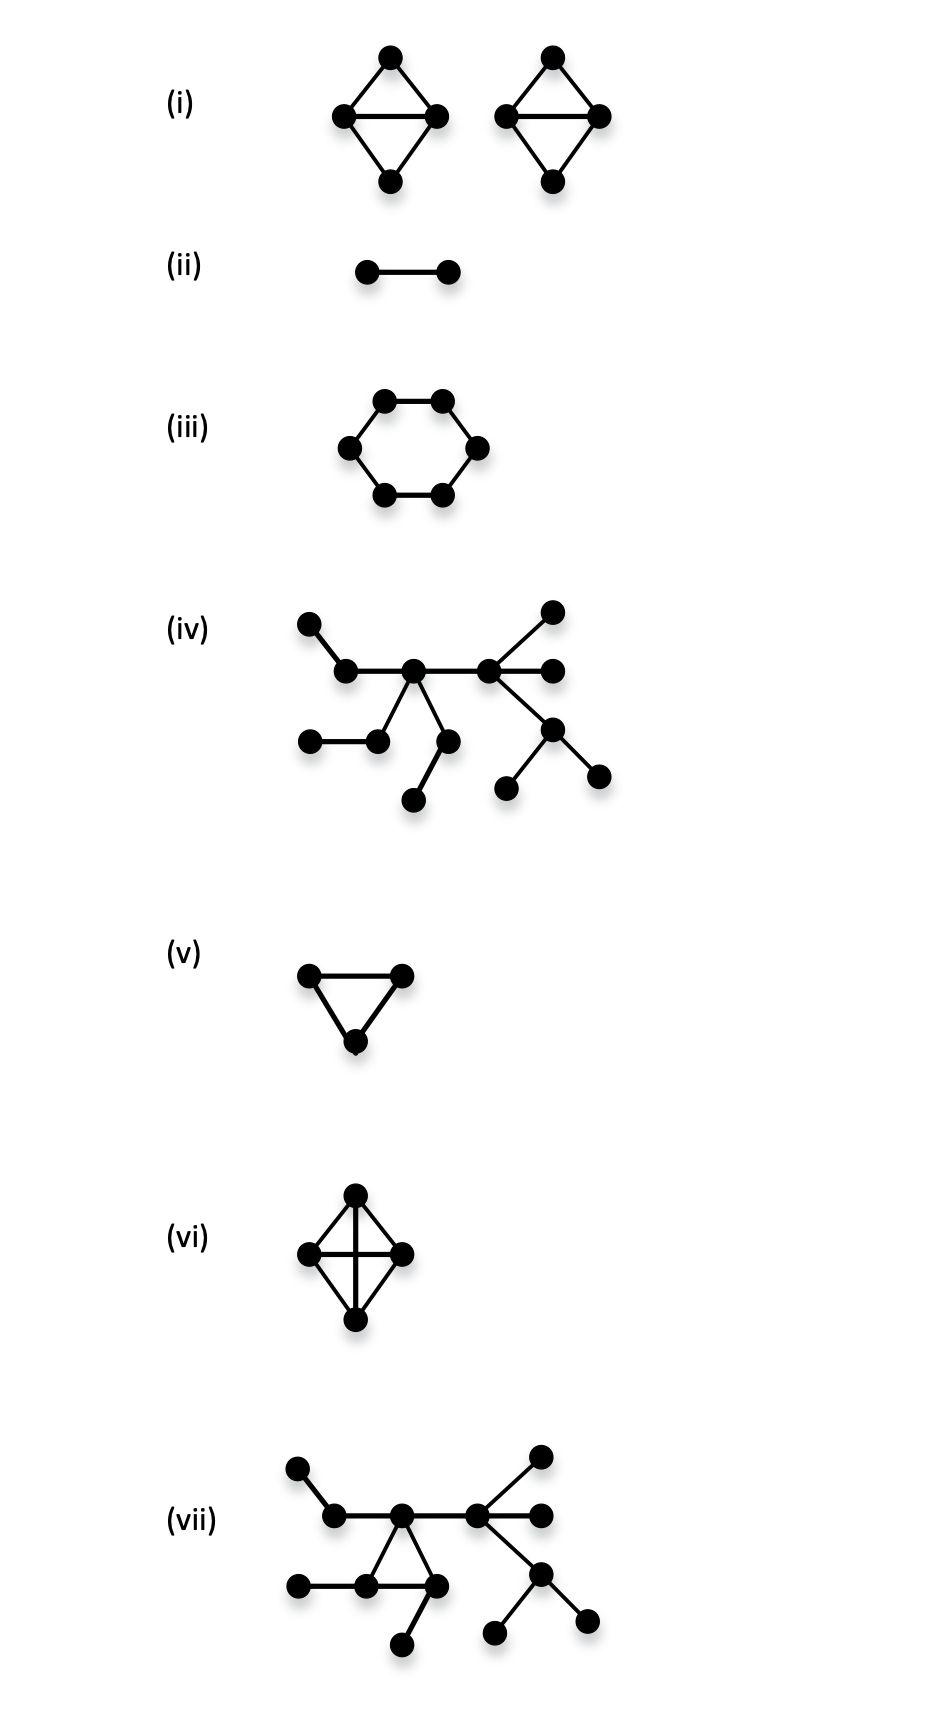
\includegraphics[width=0.5\textwidth]{p2.png}.
    \end{center}
    \begin{sol}
    \hspace*{\fill}\\
        \begin{enumerate}[i]
            \item \textcolor{red}{None}
            \item Tree, complete graph, no cycle, bipartite
            \item Not Tree, not complete graph, cycle, bipartite
            \item Tree, not complete graph, no cycle, bipartite
            \item Not Tree, complete graph, cycle, not bipartite
            \item Not Tree, complete graph, \textcolor{red}{no cycle}, not bipartite
            \item \textcolor{red}{None}
        \end{enumerate}
            \textcolor{red}{A cycle is closed walk where no vertex appears twice (except beginning and end, at least edge = points}
    \end{sol}

    %8
    \item \ [9 pts] You had a message that was 11 characters long. It was created from the letters A, B, C, D, E, F and G. You Huffman compressed the message. As a result of your compression, each letter had the following bit patterns:
    \begin{itemize}
        \item A - 0
        \item B - 110
        \item C - 111
        \item D - 1011
        \item E - 1000
        \item F - 1010
        \item G - 1001
    \end{itemize}
    \begin{enumerate}
        \item Draw the Tree that produced this compression
        \begin{sol}
        \hspace*{\fill}\\
        \begin{center}
        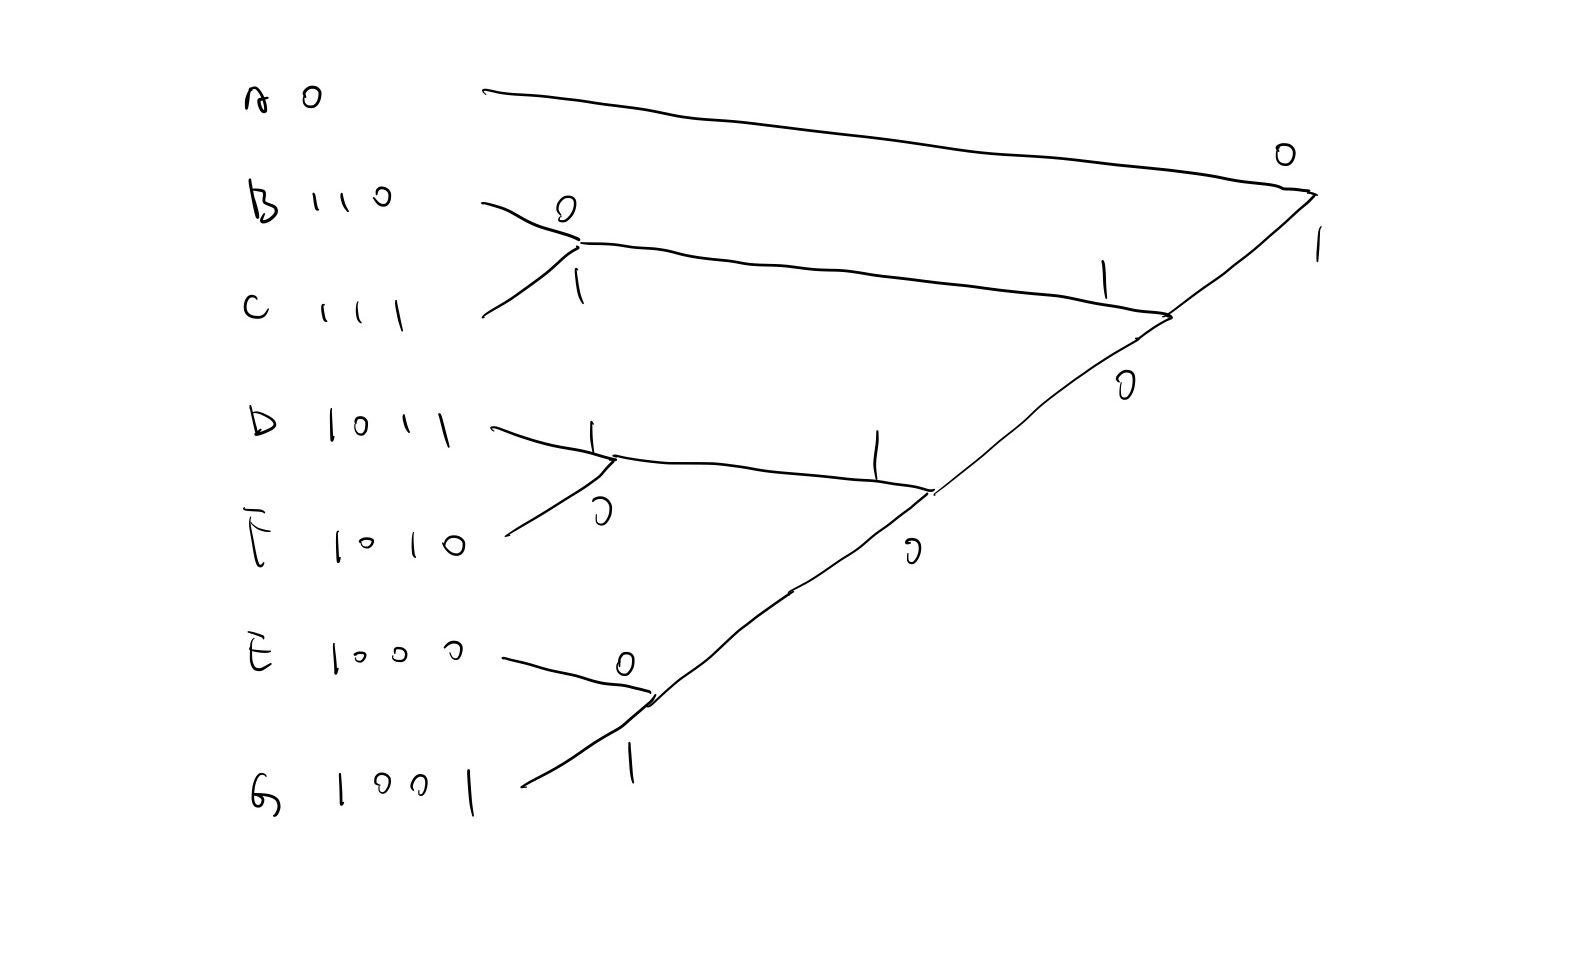
\includegraphics[width=0.9\textwidth]{p3.jpg}.
        \end{center}
        \end{sol}
        \item How many of each letter were present in the original message?
        \begin{align*}
            A: 3, B: 2, C: 2, D: 1, E: 1, F: 1, G: 1
        \end{align*}
        \textcolor{red}{
        \begin{align*}
            A: 4, B: 1, C: 2, D: 1, E: 1, F: 1, G: 1
        \end{align*}
        }
        \item How much entropy was present in the original message?
        \begin{align*}
            &3 \log_2{\frac{1}{p_A}}+4 \log_2{\frac{1}{p_B}} + 4\log_2{\frac{1}{p_D}} \\  
            &= 3 \log_2{\frac{11}{3}}+4 \log_2{\frac{11}{2}} + 4\log_2{\frac{11}{1}} \\
            &= 3 \times 1.874469118 + 4 \times 2.459431619 + 4 \times 3.459431619 \\
            & = 5.623407354 + 9.837726476 + 13.83772648 \\
            & = 29.29886031 \ bits
            & \text{other may works too}
        \end{align*}
        \textcolor{red}{
        \begin{align*}
            &4 \log_2{\frac{1}{p_A}}+1 \log_2{\frac{1}{p_B}} + 2\log_2{\frac{1}{p_C}} + 4\log_2{\frac{1}{p_D}} \\  
            &= 4 \log_2{\frac{11}{4}}+1 \log_2{\frac{11}{1}} + 2\log_2{\frac{11}{2}} + 4\log_2{\frac{11}{1}} \\
            & = 28.0537481\ bits
        \end{align*}    
        }
    \end{enumerate}

    %9
    \item \ [6 pts] A particular algorithm on a computer requires 2 seconds to process 400 items and is $\Theta(n^3)$. You want to process $8000$ items. You have a choice to either use a computer that is 10 times faster(allowing it to process 400 items in 0.2 seconds) or use the same computer with a different algorithm that still processes 400 items in 2 seconds, but has a growth rate that is $\Theta(n^2)$
    \begin{enumerate}
        \item Which is the faster choice for 8000 items?
        \begin{sol}
        \begin{align*}
            & \text{faster computer: \ } time = (\frac{8000}{400})^3 \times 0.2 = (20)^3 \times 0.2 = 1600 \ seconds\\
            & \Theta(n^2) \text{ \ algorithm: \ } time = (\frac{8000}{400})^2 \times 2 = (20)^2 \times 2 = 800 \ seconds\\
            & \therefore \Theta(n^2) \text{ \ algorithm better for 8000 items } 
        \end{align*}
        \end{sol}
        \item For what input sizes is the faster computer better?
        \begin{sol}
        \begin{align*}
            & \text{suppose input sizes is \ } n\\
            & (\frac{n}{400})^3 \times 0.2 < (\frac{n}{400})^2 \times 2 \rightarrow n < 4000\\
            & \therefore \text{when the input sizes is smaller than 4000}
        \end{align*}
        \end{sol}
        \item For what input sizes is the $\Theta(n^2)$  algorithm better?
        \begin{sol}
        \begin{align*}
            \text{When the input sizes is larger than 4000.}
        \end{align*}
        \end{sol}
    \end{enumerate}

    % 10
    \item \ [9 pts] Consider two different algorithms that each solve a different problem.
    \begin{itemize}
        \item Algorithm X solves Problem $P_x$ and Algorithm X is $O(n^3)$ and $\Omega(n)$
        \item Algorithm Y solves Problem $P_y$ and Algorithm Y is $O(n^4)$ and $\Omega(n^2)$
        \item Algorithm Z solves Problem $P_z$ and Algorithm Z is $\Theta(n^5)$

        From the information above, determine if each of these `` \textbf{Yes} it is true ", ``\textbf{Maybe} it is true but doesn't have to be", or `` \textbf{No} it is not true".
    \end{itemize}
    \begin{enumerate}
        \item Problem $P_y$ is harder than Problem $P_z$ : M
        \item Problem $P_z$ is harder than Problem $P_x$ : M
        \item Algorithm Y is harder than Algorithm X : \textcolor{red}{M} %Y
        \begin{sol}
            Because the Algorithm X is between $O(n^3)$ and $\Omega(n)$, Algorithm Y is between $O(n^4)$ and $\Omega(n^2)$. They can be $n^3$ at the same time, which means may be. 
        \end{sol}
        \item Problem Y is $\Omega(n^2)$ : \textcolor{red}{M} % N
        \begin{sol}
            Because the Algorithm Y is $O(n^4)$ and $\Omega(n^2)$, the problem the worst must be equal or less than Algorithm. Therefore, the Problem Y is $\Omega(n^2)$ or $\Omega(n)$... 
        \end{sol}
        
        \item Problem X is $\omega(\log n)$: M
        \item Problem Y is $O(n^4)$: Y
        \item Problem X is $o(n^4)$: \textcolor{red}{Y} %N
        \begin{sol}
            Because the Algorithm X is $O(n^3)$ and $\Omega(n)$, therefore, the problem X must equal or less $O(n^3)$. Therefore, if $o(n^4)$ is ok.
        \end{sol}
        \item Algorithm Z is $\Omega(n)$: Y
        \item Algorithm Z is $w(n)$: Y
        
    \end{enumerate}

    % 11
    \item \ [10 pts] Setup the table as shown in class and determine 1/10 modulo 7657.
    \begin{sol}
        \hspace*{\fill} \\
        \begin{center}
            \begin{tabular}{|c|c|c|c|c|c|c|c|c|}
                 \hline
                 $\bmod \ 7657$ & 1 & 2 & 3 & 4 & 5 & 6 & 7  \\
                 \hline
                    7657  &  7657 +1 =7658& 2 \times 7657+1 = 15315 &22972 &  30629 & 38286 & 45943 & 53600  \\
                 \hline
            \end{tabular}
        \end{center}
        \textcolor{red}{
        \begin{align*}
            & (53600) \bmod 7657 = (5360 \times 10 ) \bmod 7657 = 1 \\
            & (\frac{1}{10} \times 10 ) \bmod 7657 = 1  \\ 
            & (\frac{1}{10}) \bmod 7657 = 5360 \\
            & 
        \end{align*}
        }
    \end{sol}

    % 12 
    \item \ [6 pts] Solve the following for the value of A. Ensure your answer is an integer between 1 and 3058 inclusive.
    \begin{align*}
        1822 = ((5*A) + 89) \ modulo \ 3059
    \end{align*}
    \begin{sol}
    \begin{align*}
        & ((5*A) + 89) \bmod  3059 = 1822 \\
        & (5 * A) \bmod 3059 = 1822 - 89 \\
        & (5 * A) \bmod 3059 = 1733 \\ 
        & \therefore (5*A) = B \times 3059 + 1733 \\
             &  A = \frac{B\times 3059 +1733}{5} \\
             & \because \text{A is integer, and B is also integer} \\
             & \therefore A = 2182
    \end{align*}
    \end{sol}

    % 13
    \item \ [6 pts] You have the following graph:
        \begin{center}
        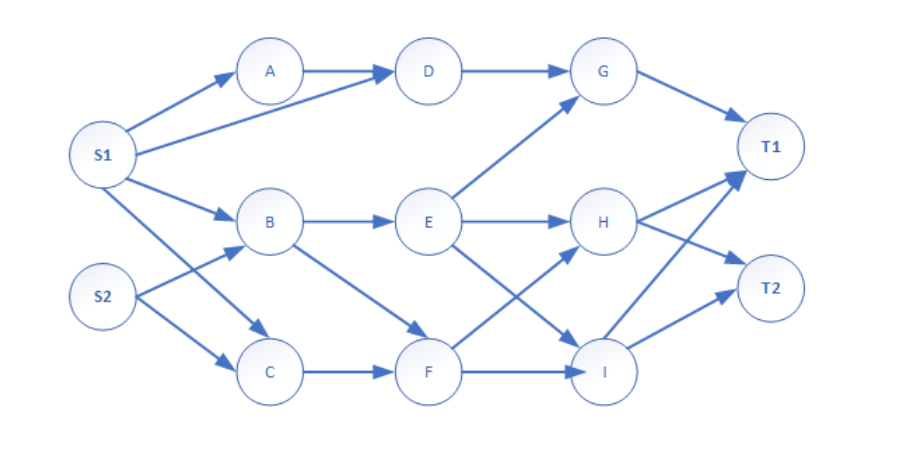
\includegraphics[width=0.8\textwidth]{p4.png}.
        \end{center}
    Assume each of the edges have numbers associated with them that represent the flow of goods. You can think of S1 and S2 as being warehouses that need to be emptied and you can think of T1 and T2 as being storage facilities that can store the items from the S1 and S2 warehouses which are being emptied. Items leaving the S1 and S2 warehouses can be split between the T1 and T2 storage facilities. That is, you do not care which storage facility T1 or T2 each item arrives at. You just want to empty them from S1 and S2 as fast as possible. 
    
    How would you modify the graph above to allow you to use the Ford-Fulkerson maximum flow algorithm we learned in class that works for a single source, S, and a single sink, T, to solve this problem?
    \begin{sol}
                \begin{center}
        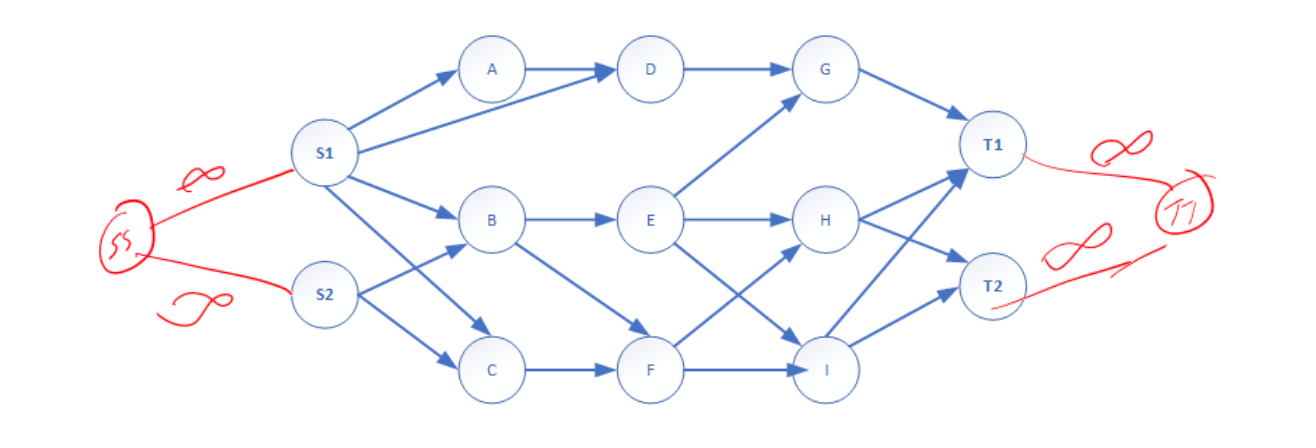
\includegraphics[width=0.8\textwidth]{p6.png}.
        \end{center}
    \end{sol}
    
    % 14
    \item \ [6 pts] Draw a graph and give a smallest last vertex ordering where the terminal clique is not the largest complete subgraph. Circle the first vertex you write down in your smallest last ordering.
    \begin{sol}
        \begin{align*}
            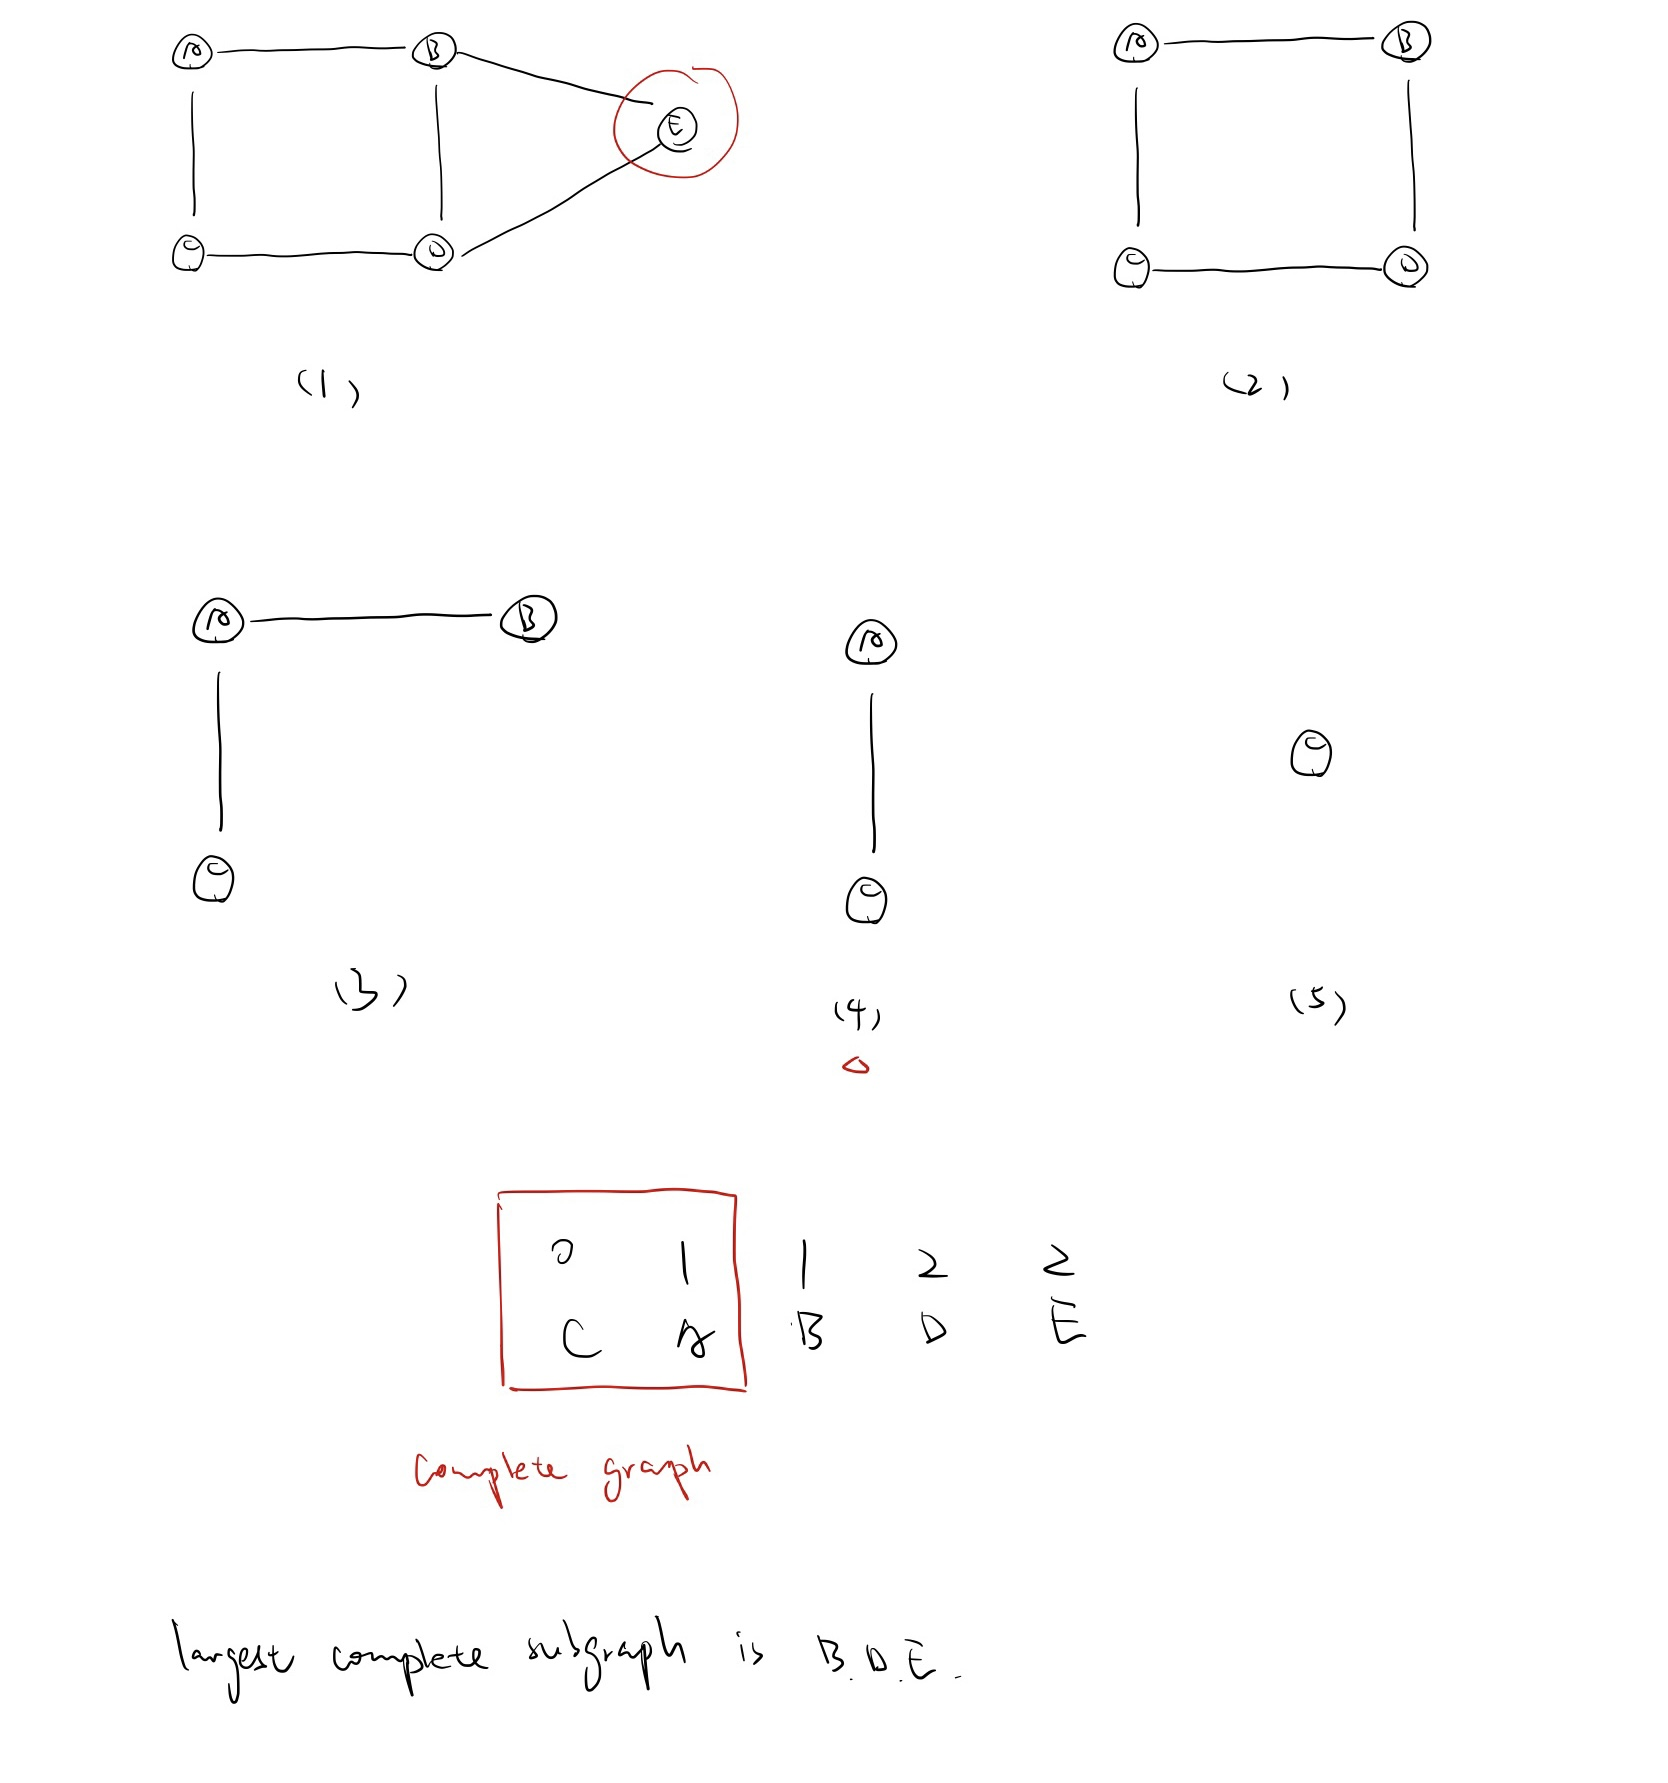
\includegraphics[width=0.8\textwidth]{p5.jpg}.
        \end{align*}

    \end{sol}
    
    % 15
    \item \ [6 pts] Answer the following questions:
    \begin{enumerate}
        \item What is the weight of a minimum spanning tree for a connected, acyclic graph with $|V|$ vertices where all edges have a weight of 4?
        \begin{sol}
            $4(|V|-1)$
        \end{sol}
        \item What is the weight of a minimum spanning tree for a cycle with 10 vertices where all edges have a weight of 4?
        \begin{sol}
            $4(|V|-1) = 4 \times (10-1) = 36$
        \end{sol}
        \item A complete bi-partite graph $B_{j,k}$ is a graph which has J vertices in one partition and k vertices in another partition and all possible edges present between the partitions. For which values of j and which values of k are the degrees of the vertices even?
        \begin{sol}
        \hspace*{\fill}\\
        If j is even, then the degree K vertices are even.\\
        If k is even, then the degree J vertices are even.\\
        \textcolor{red}{When j,k are both even.}
        \end{sol}
    \end{enumerate}
    \begin{align*}
    \end{align*}
\end{enumerate}
\end{document}
